\subsection{研究内容}\label{ch2content}

本项目面向医疗卫生行业的数据分析需求,针对电子医疗记录分析存在的研究队列识别困
难、记录时间不规则、模型解释匮乏等问题,以深度学习为基础手段,研究电子医疗记录分
析建模的理论和方法,力争构建端到端的电子医疗记录分析方案,突破队列识别、EMR插补
和可解释性分析模型等关键技术,并在基于电子医疗记录的临床任务上验证本项目的研究成
果。

项目研究工作从队列识别、EMR插补、可解释分析模型和临床任务验证四个层次展开,本项
目的挑战、科学问题和研究内容关系如图~\ref{fig:ch2:rc}所示。各部分研究内容具体介
绍如下:

\begin{figure}[htp]
    \begin{small}
        \begin{center}
            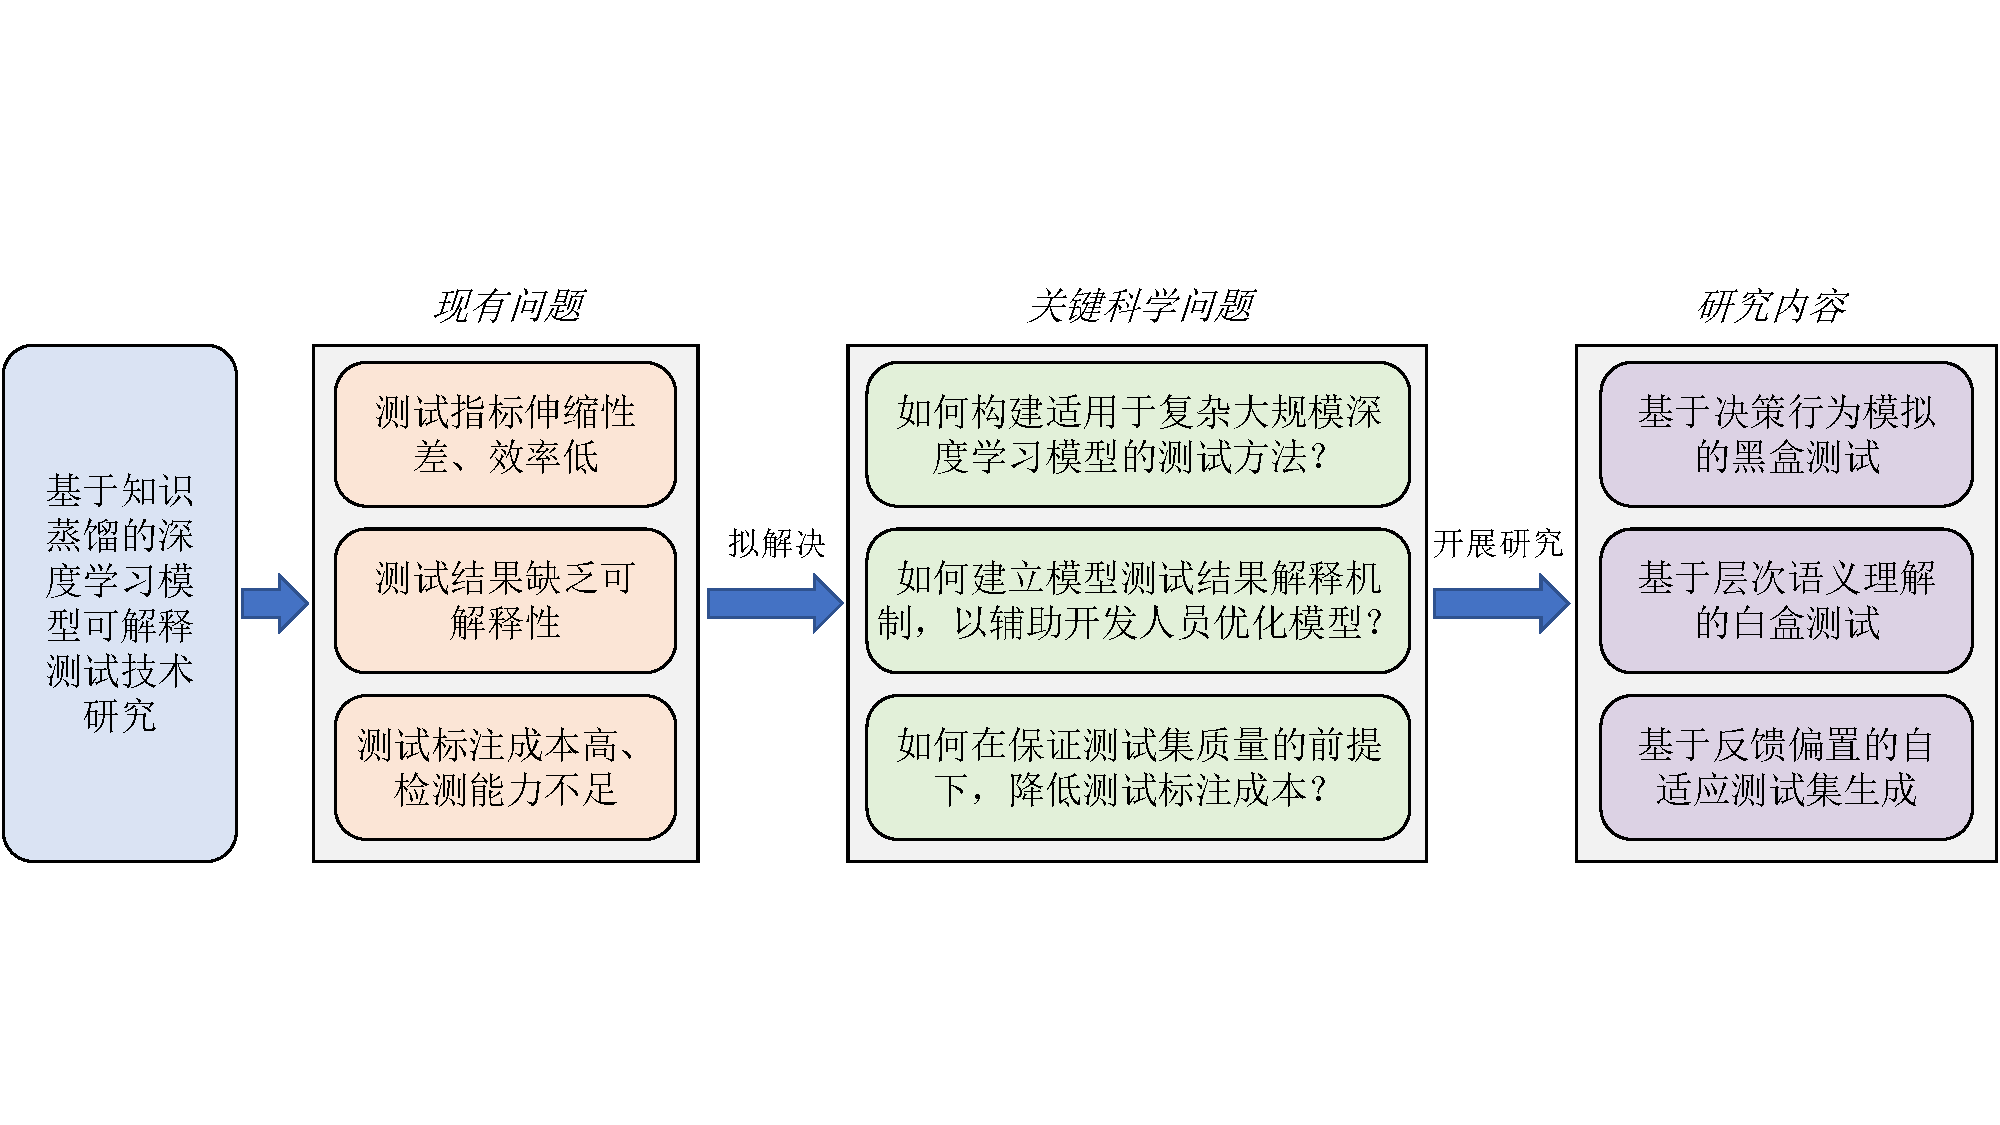
\includegraphics[width=0.95\textwidth]{ch2_framework.pdf}
        \end{center}
        \caption{挑战、科学问题和研究内容关系图}
        \label{fig:ch2:rc}
    \end{small}
\end{figure}

\subsubsection{基于决策行为模拟的黑盒测试}

借鉴传统软件的路径覆盖测试方法,许多研究提出针对深度学习模型的覆盖性测试方法(参
见\ref{relatedwork} 国内外研究现状及发展动态分析),这些测试覆盖指标和方法主要是
针对白盒的场景,即测试者掌握所有的训练数据和整个深度学习模型,\textbf{但在许多场
景中,测试者无法访问训练数据和模型内部结构,但仍需要对模型的泛化能力进行测试,即
黑盒测试,如深度学习模型是某个公司私有的或者由第三方机构提供,他们只提供了接口或
者打包的可执行程序。}因此,本项目面向黑盒测试场景,研究基于决策行为模拟的黑盒测
试方法。

以分类模型为例,给定一个黑盒深度学习模型$\mathcal M$和测试数据集$\mathcal
D_{\text{test}}=\{x^{(i)},y^{(i)}\}$,测试者可以得到模型针对每个输入
$x^{(i)}$(input)的输出$\hat{y}^{(i)}$,通常是该输入属于各个类别的概率分布,除
此之外,测试者无法知道该模型的训练数据和内部结构。可见,深度学习模型黑盒测试面临
两个主要问题:
\begin{itemize}
    \item \textbf{如何建立模型有关的测试方法?}仅有的几个黑盒模型测试方法仅针对
    数据的多样性进行评估,无法准确反映模型的泛化能力,也不能给模型改进提供有效建
    议。
    \item \textbf{如何掌握模型的决策机制?}黑盒测试无法了解模型的结构,难以掌握模型的决策机制。
\end{itemize}

\begin{figure}[htp]
    \begin{small}
        \begin{center}
            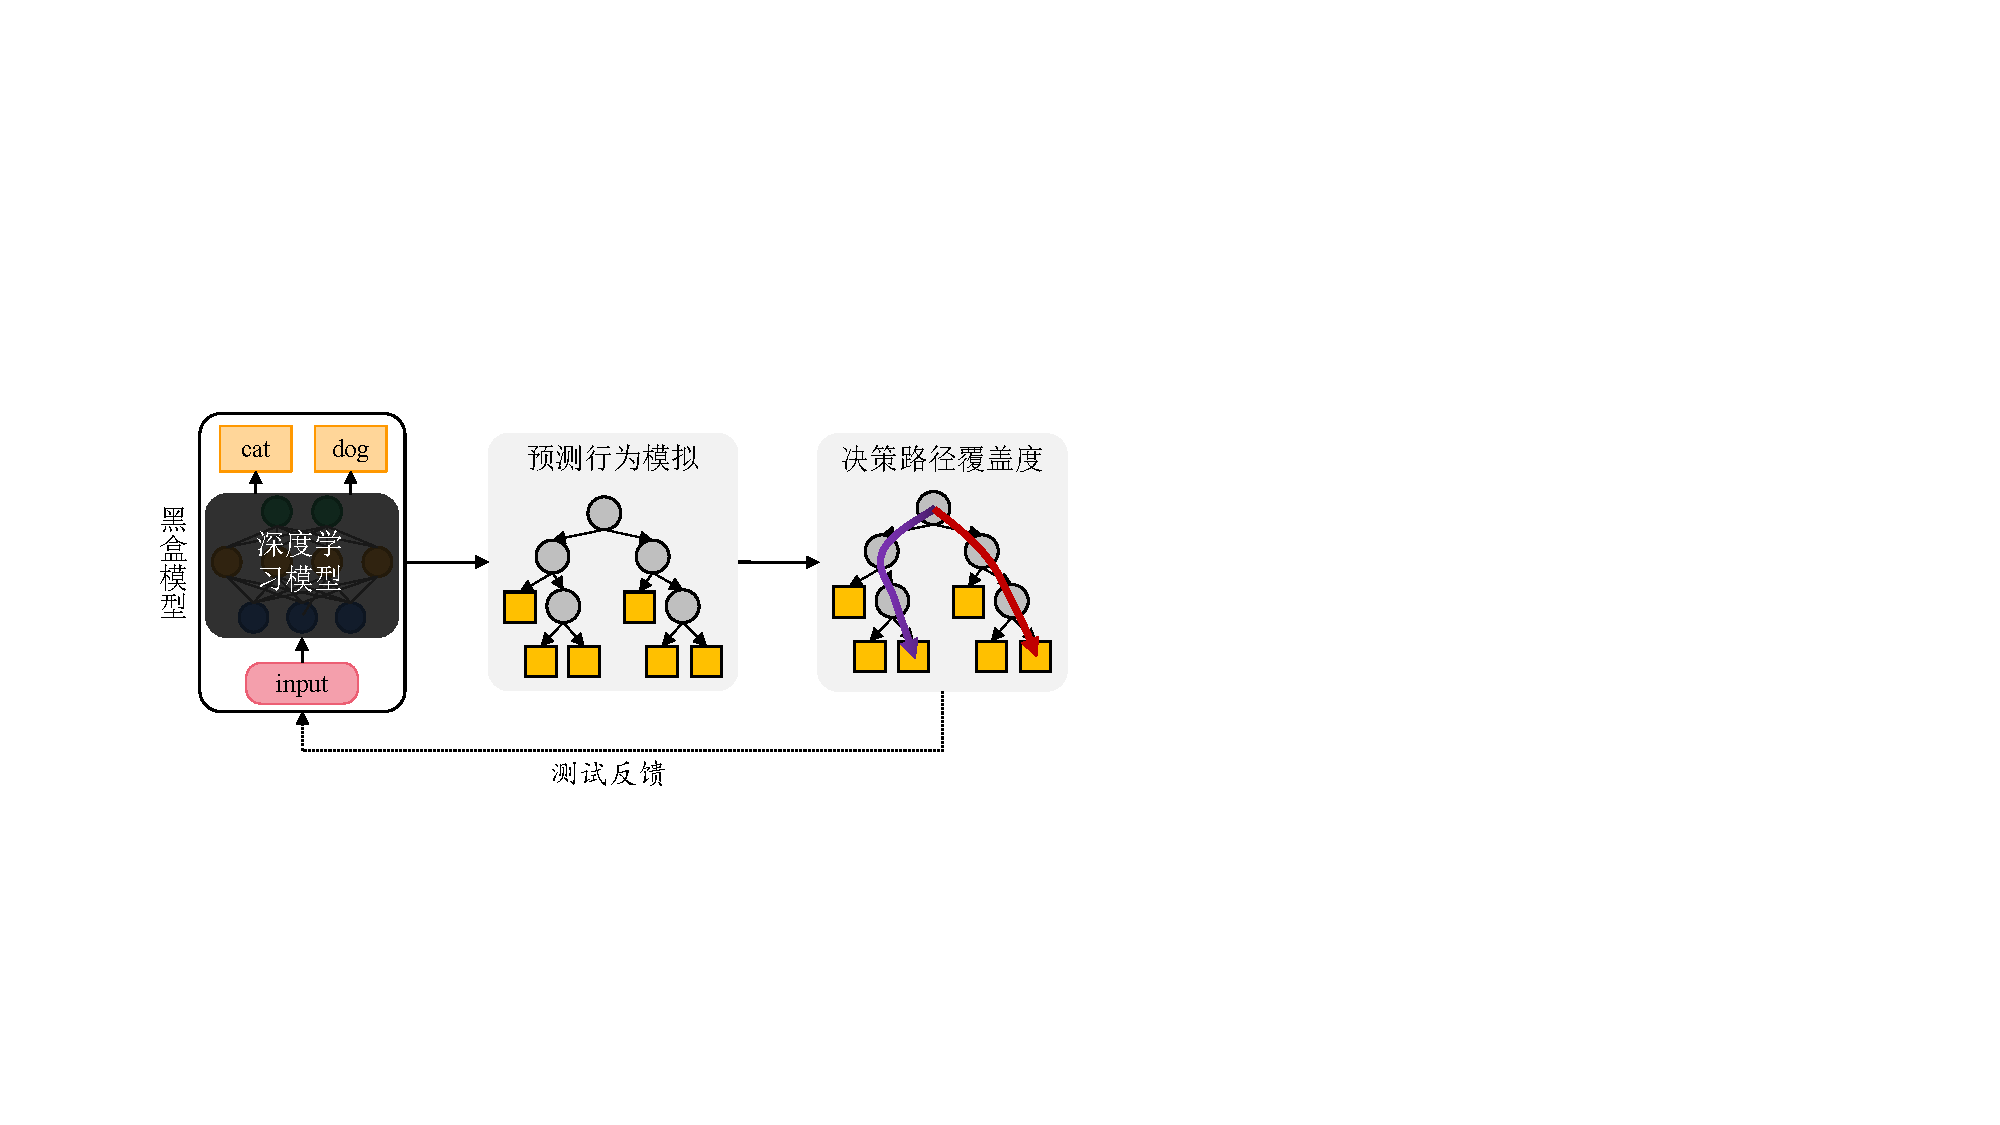
\includegraphics[width=0.8\textwidth]{ch2_2Btest.pdf}
        \end{center}
        \caption{基于决策行为模拟的黑盒测试研究内容}
        \label{fig:ch2:2Btest}
    \end{small}
\end{figure}
本项目深度学习模型黑盒测试的主要研究内容如\cref{fig:ch2:2Btest}所示,\textbf{本项目首先
研究针对黑盒模型的预测行为模拟方法,拟利用知识萃取的方法,通过建立副本模型
$\mathcal M^\prime$(如决策树)萃取黑盒模型$\mathcal M$的知识,模拟$\mathcal M$
的预测行为;然后,在副本模型的基础上,本项目拟建立基于决策路径覆盖度的测试方法,
通过覆盖度指标反映模型的决策机制和泛化能力。}

\subsubsection{基于层次语义理解的白盒测试}

除了黑盒测试的场景,白盒测试的需求也非常多,如企业自己开发的深度学习模型,在白盒
测试中,测试者可以访问模型的内部结构$\mathcal M(\bm W, \bm b)$和训练数据集
$\mathcal D_{train}=\{(x^{(i)}, y^{(i)}\})$。目前,针对深度学习模型的白盒测试方
法可扩展性和可解释性较差,无法应用于大规模深度学习模型,如
BERT~\cite{kenton2019bert},MAE~\cite{he2021masked}等,而且测试结果无法给模型训
练提供有效反馈,辅助模型优化。因此,\textbf{本项目提出针对白盒深度学习模型的层次
语义理解方法,通过知识蒸馏技术将各层的决策语义融入``学生''模型中,保证``学生''模
型的决策路径与原白盒模型一致;然后围绕``学生''模型进行决策路径覆盖度测试,决策路
径具有较强的可解释性,可引导测试数据生成和模型优化。}

\begin{figure}[htp]
    \begin{small}
        \begin{center}
            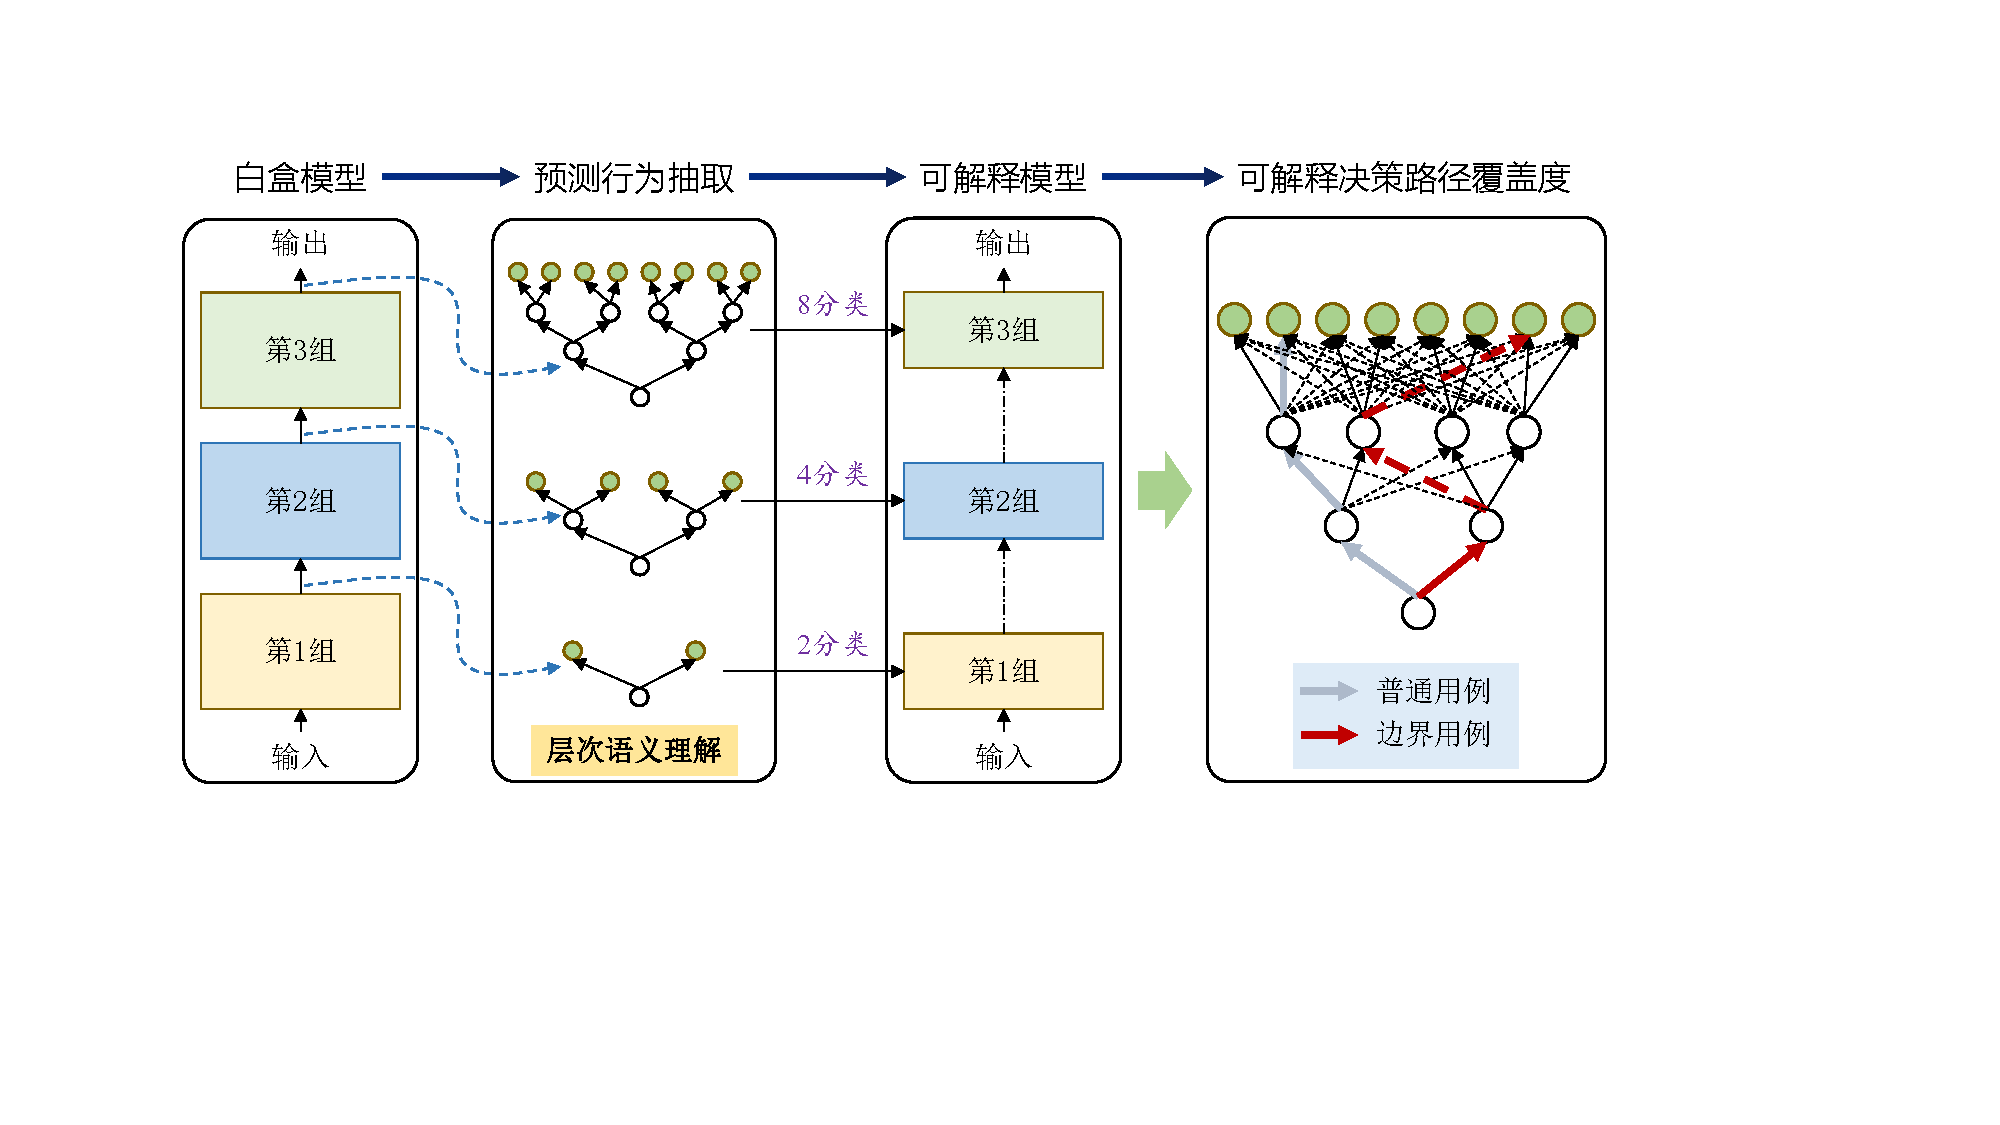
\includegraphics[width=0.9\textwidth]{ch2_WBtest.pdf}
        \end{center}
        \caption{基于层次语义理解的白盒测试研究内容}
        \label{fig:ch2:WBtest}
    \end{small}
\end{figure}

本项目基于层次语义理解的白盒测试研究内容如\cref{fig:ch2:WBtest}所示,在白盒测试
的场景下,本项目首先研究如何从深度学习模型中抽取出各层(layer)的决策语义信息,
研究表明,深度学习模型对输入的决策是由粗粒度到细粒度的。\cref{fig:ch2:WBtest}举
例说明了从3组神经网络层的输出抽取各组网络的预测行为,例如:输入一个猫的图片,第1
组神经网络判断该图片是否是动物,接着,第2组神经网络判断该图片是否是猫科动物,最
后,第3组神经网络将该图片分类为猫。\textbf{本项目拟研究如何实现层次语义理解,自
动地从深度学习模型中抽取出各层的决策语义}。

在层次语义理解的基础上,\textbf{本项目拟利用知识蒸馏技术训练一个``学生''模型,通
过融入原白盒模型的决策语义,使知识蒸馏得到的``学生''的决策路径与原白盒模型一致,
且具有良好的可解释性}。此外,知识蒸馏得到的模型通常规模较小,和直接测试原白盒模
型相比,测试``学生''模型可有效提高测试效率。\textbf{在得到可解释的``学生''模型
后,本项目拟研究并提出针对该可解释模型的决策路径覆盖度,用于分析测试样本的多样性
和充分性}。


\subsubsection{结合特征重要性和时间关联性的可解释预测模型}

如图~\ref{fig:ch2:interpretability}所示,电子医疗记录除了包含随时间变化的医疗特
征,还会包含患者的人口统计学特征,如性别、种族等,这些特征虽然是静态不变的,但对
预测患者病情发展也非常重要,所以\textbf{在构建预测模型时,首先应该研究如何将患者
的静态特征和动态特征分别建模,以及如何融合两组特征进行分析}。

\begin{figure}
    \begin{small}
        \begin{center}
            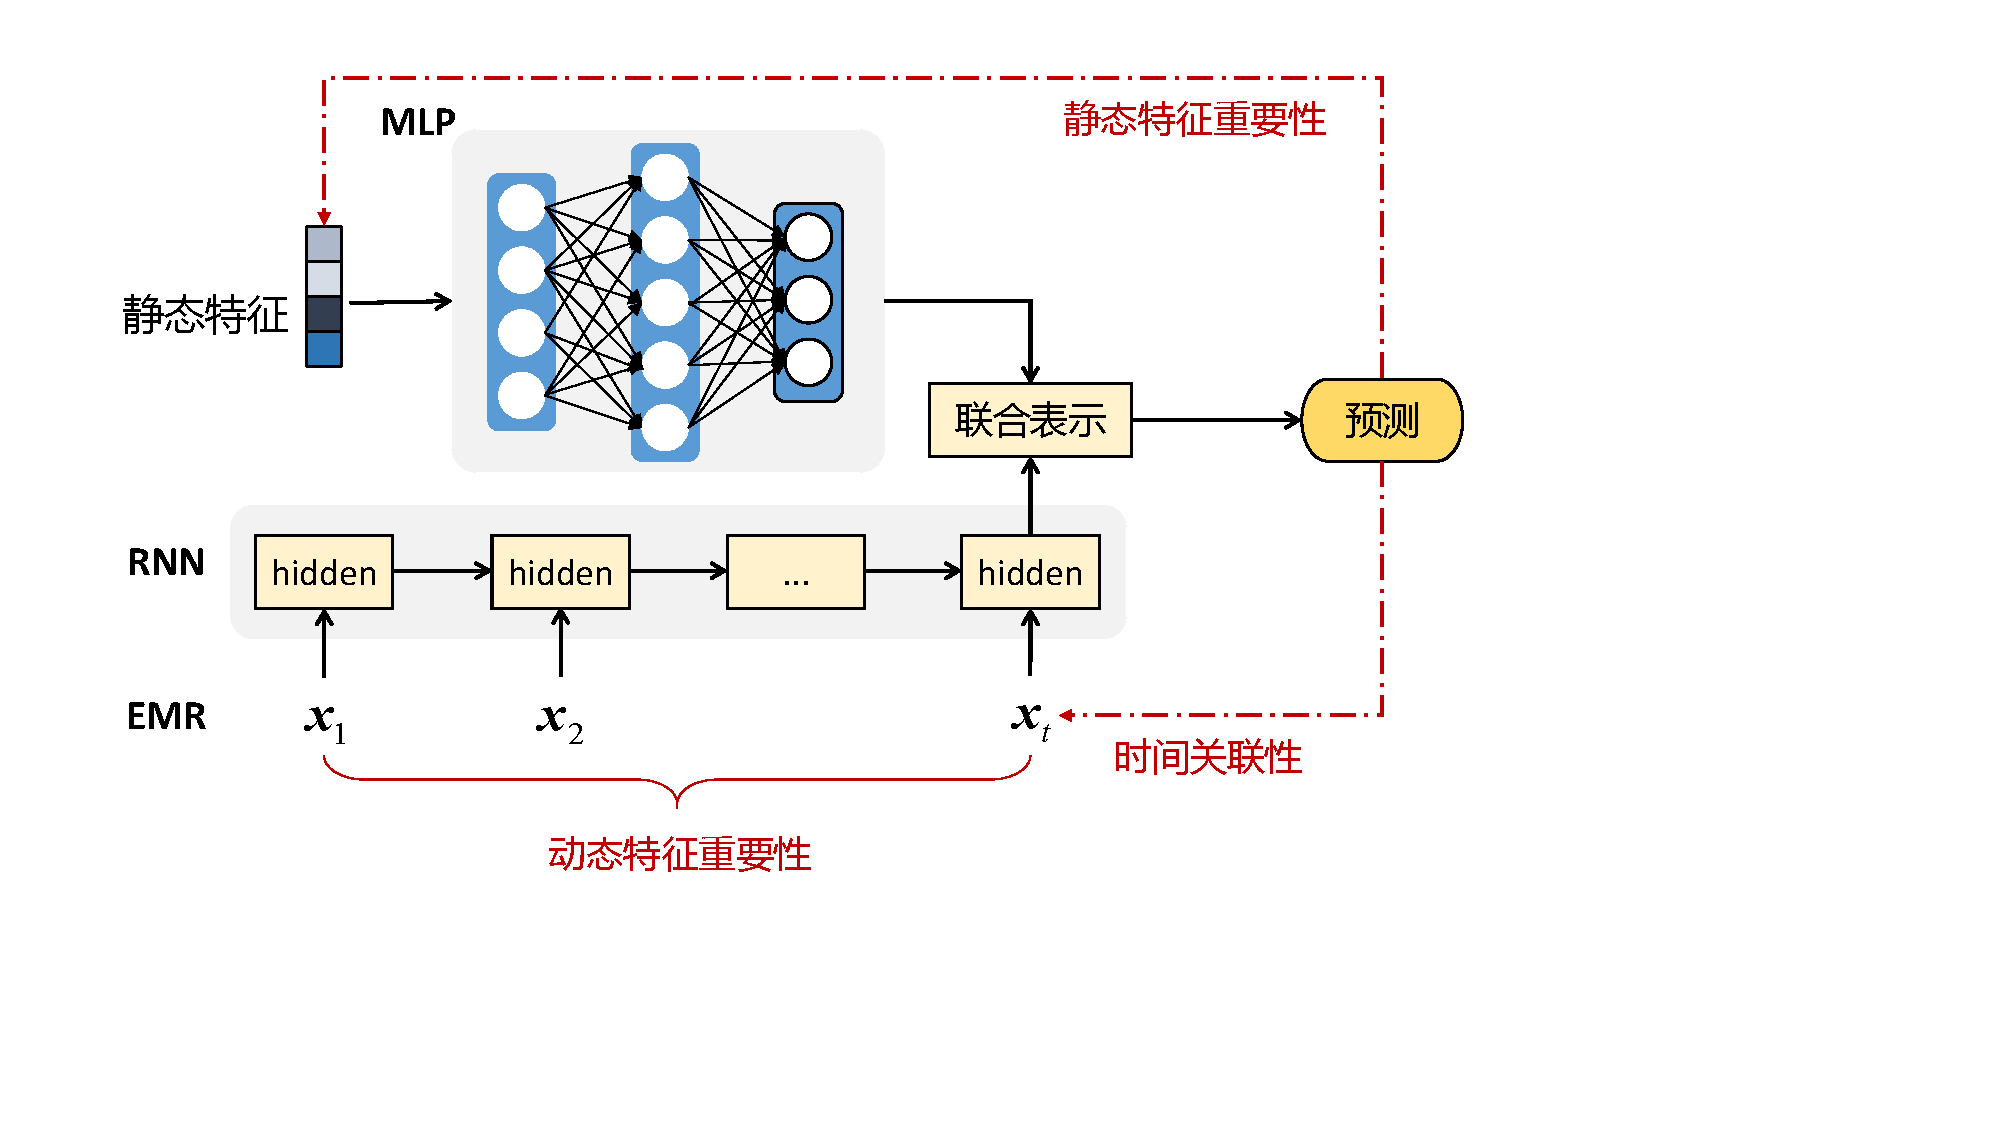
\includegraphics[width=0.75\textwidth]{ch2Interpretability.pdf}
        \end{center}
        \caption{可解释预测模型研究内容}
        \label{fig:ch2:interpretability}
    \end{small}
\end{figure}

模型的临床应用需要提供对模型和预测结果的解释,因此,预测模型的可解释性是本项目另
一个重要的研究内容。目前用于电子医疗记录分析的可解释方法可分为两类:第一类研究在
预测模型建模时没有考虑其解释性,但利用后解释(post-interpretable)模型来解释预测
结果,这类方法具有两个缺点,一是后解释模型把任何预测模型当作黑盒,依然无法让医生
了解模型真实的决策过程,只能提供预测结果的可靠程度,二是随着就诊数据的变化,需要
重新训练预测模型和后解释模型,带来了额外开销;第二类研究在预测模型中实现可解释
性,在完成预测的同时,也能为预测结果提供可解释的依据,这类方法尝试在预测准确性和
可解释性两方面找到一种平衡,通常在模型实现可解释性时,其准确率会有所下降。

本项目拟在预测模型中考虑可解释性,现有工作缺少对静态特征和动态特征的统一比较,无
法得到模型的全局可解释性。静态特征通常用浅层全连接层建模,本项目拟采用逐层相关性
传播~\citess{bach2015pixel}分析静态特征与预测结果的关系。而对动态特征,本项目拟
采用RNN模型进行建模,但由于RNN复用隐含层,其针对多维特征的可解释特别差,一方面,
隐含层是由所有特征经过多步计算得到的,无法从隐含层解耦出每个特征对预测结果的贡
献;另一方面,RNN中最后的隐含层是由多步计算得到,其时间信息也无法逆向得到,阻碍
了特征出现时间的分析。所以动态特征可解释性研究的重点在于分析高维的动态特征与预测
目标的关系。\textbf{本项目通过对RNN隐含层解耦,挖掘动态特征重要性和时间关联性,
并统一比较动态特征和静态特征的贡献,实现模型的全局解释,且可回溯样本预测结果,为
医务人员提供全面的模型解释}。

\subsubsection{临床预测性任务}

\textbf{本项目拟将研究成果应用于具体的临床预测性任务,以验证其有效性,同时,通过
和临床医生的合作,提高研究质量,加速研究成果应用}。具体而言,本项目拟将研究成果
应用于慢性肾脏病进展预测和急诊科感染性休克预警,并通过和医生的交流,保证项目研究
内容具有实际应用价值。

\begin{itemize}
    \item  \textbf{与北京大学医疗健康大数据国家研究院合作,预测DKD慢性肾病患者的
    病情发展情况},提醒医生及时进行临床干预。
    \item  利用机器学习手段预测病人状态对降低ICU感染性休克的病发率和死亡率具有重
    要意义。\textbf{本项目拟基于MIMIC-III~\citess{johnson2016mimic},利用项目研
    究成果实现ICU患者感染性休克预警系统},验证项目研究成果的有效性。
\end{itemize}


\subsection{研究目标}\label{ch2target}

本项目从医疗卫生行业和人工智能结合的实际需求出发,针对队列识别泛化能力差、EMR插
补准确率低、以及预测模型可解释性匮乏等问题,研究队列识别、EMR插补和可解释预测模
型等问题,并将相关研究成果应用实际临床数据,检验本项目的研究成果在电子医疗记录预
测性分析中的应用效果,推动电子医疗记录分析的研究进展。

具体研究目标包括:

\textbf{在技术方面},本项目拟在以下四方面实现技术突破: (a) 提出基于表现型的队列
识别方法,充分利用已标注和未标注数据,提高队列识别模型的准确性和表示学习的泛化能
力;(b) 提出融合医学偏差的EMR自动插补方法,实现数据预处理,通过合理引入医学偏
差,提高EMR插补的准确性;(c) 提出可解释预测模型,在进行预测的同时,可以从模型中
得到与预测目标相关的特征和时间点;(d) 将本项目的研究成果应用于DKD患者病情进展预
测和重症监护室患者感染性休克预测。

\textbf{在成果形式方面},本项目力争在国内外高水平期刊、会议上发表论文8篇以上,全
部被SCI/EI检索,其中有重要影响的论文4篇以上;申请专利2项。

\textbf{在人才培养方面},通过本项目研究,培养深度学习、电子医疗记录分析、可解释人工智能等交叉领域的青年人才,拟培养研究生3-4人。

\subsection{拟解决的关键科学问题}

基于上述研究目标和研究内容,本项目拟在以下几个关键理论和技术问题上有所突破:

\subsubsection{在弱监督条件下构建泛化性强的患者层次表示,实现自动队列识别}

从海量、高维的电子医疗记录中识别研究队列是电子医疗记录分析的基础,由于电子医疗记
录的高维性和表现型的组合性,依靠医务人员人力筛选和标注所有符合预定表现型的队列数
据不具有可操作性。患者的表现型表示可以更准确地对应预定义表现型,提高队列识别准确
度,但仅基于少量队列标签的EMR数据集不足以让模型学习到好的数据分布,同时,传统半
监督方法在标注数据和未标注数据上分别训练,模型的训练更容易被未标注数据影响。因
此,如何合理利用大量未标注数据辅助建模,构建泛化性强的患者层次表示,实现电子医疗
记录的队列识别是本项目拟解决一个关键科学问题。

\subsubsection{建立医学偏差和缺失矩阵的对应关系,并将其融入电子医疗记录插补中}

电子医疗记录具有时间不规则性,直接在电子医疗记录上建模和训练难以得到较好的结果,
训练得到的模型通常容易过拟合,泛化性较差。在构建预测模型之前对电子医疗记录进行插
补具有重要意义,可以降低预测模型复杂度和训练难度。现有方法忽略了电子医疗记录中固
有的医学偏差,将其中的缺失值当作完全随机缺失对待,其插补结果不够准确。医学偏差并
不是数据质量问题或者噪声,反而对充分理解电子医疗记录非常重要。如何建立医学偏差和
记录缺失的对应关系,并将其融合到电子医疗记录插补中是本项目构建通用电子医疗记录处
理框架要解决的一个关键科学问题。

\subsubsection{融合特征重要性和时间关联性,建立电子医疗记录可解释分析模型}

模型的可解释性对医学领域的预测性分析至关重要,决定了模型是否能应用于临床实践。电
子医疗记录(动态特征)是一种特殊的多元时序数据,通常采用RNN模型建模,但在RNN学习
过程中,多个特征在不同时间点的取值都被糅合在RNN的隐含层中,无法总结得到特征对于
模型的意义,也无法计算出某条记录和预测结果的相关性。因此,如何融合特征重要性和时
间关联性,构建可解释预测模型,支持模型的全局解释和预测结果的回溯,也是本项目拟解
决的一个关键科学问题。